\begin{figure}[ht!]
\centering
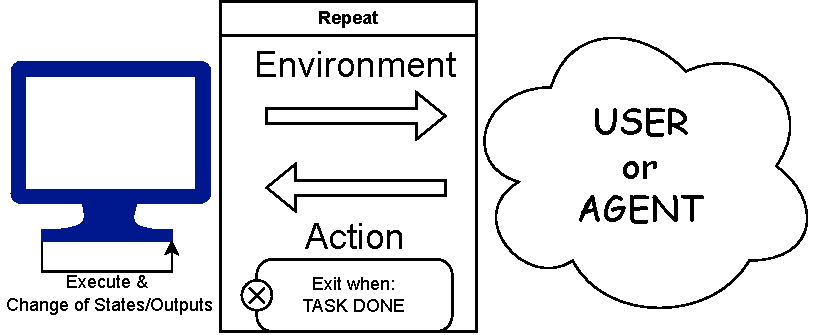
\includegraphics[width=\linewidth]{Figures/pre-Computer's perspective.drawio.pdf}
\caption{An illustration of why we use computers.}
\label{fig:why-use-computer}
\end{figure}

\section{The Computer Use Agent: Eyes, Brains, and Hands}
% \label{sec:intro}

The capacity of Large Language Models (LLMs) to reliably function as Computer Use Agents (CUAs)~\cite{DBLP:conf/cvpr/HongWLXYJWWD0024, 10.5555/3692070.3694608} is underpinned by two principal technological advancements: the integration of \textbf{Vision-Language Models (VLMs)}~\cite{DBLP:conf/icml/RadfordKHRGASAM21, 10.5555/3692070.3694608} and the implementation of robust, constrained \textbf{function calling} mechanisms.

Vision-Language Models function as the perceptual and cognitive components of the agents. While conventional LLMs produce semantically coherent textual output, advanced \textbf{reasoning models}~\cite{DBLP:conf/nips/Wei0SBIXCLZ22, DBLP:journals/corr/abs-2305-20050} (e.g., Gemini 3 Pro, OpenAI o3, and Deepseek-R1) exhibit significantly enhanced logical capabilities and strategic planning. Critically, as human-computer interaction is predicated upon visual modalities, the overwhelming volume of screen-based information, including UI structures and fonts, images and video, is not amenable to direct textual conveyance. This disparity is addressed through the employment of \textbf{image encoders}~\cite{DBLP:conf/iclr/DosovitskiyB0WZ21} (e.g., Vision Transformers, or ViTs) and \textbf{projectors}~\cite{DBLP:conf/iclr/DosovitskiyB0WZ21, DBLP:conf/nips/LiuLWL23a}, which facilitate the necessary alignment of visual data with the established linguistic domain. Consequently, VLMs are endowed with the capacity to comprehensively perceive and interpret the desktop environment, thereby providing a foundation for responsive interaction with the operational state of the machine.

The capacity for autonomous action requires a reliable mechanism for \textbf{execution}. Given that natural language is inherently descriptive rather than executable, agents are necessitated to interface with structured programming environments using specific syntax, generally realized through a function call. Although various tools can be provided to the agent, the inherent \textbf{stochasticity}~\cite{DBLP:conf/acl/LewisDF18, DBLP:conf/iclr/HoltzmanBDFC20} of conventional LLM token sampling often introduces instability, resulting in syntactical errors within the generated output. To mitigate this pervasive issue, models are prompted to output a serialized object, typically \textbf{JSON}, which formally represents the function call. While optimization via system prompts and model fine-tuning can improve format adherence, these methods do not structurally guarantee correctness. Consequently, the stability of execution relies on the application of \textbf{grammar-based sampling} techniques during the inference process. As JSON is formally defined by \textbf{Context-Free Grammars (CFG)} \cite{10.17487/RFC8259}, a formal parser is used to dynamically construct a finite set of grammatically permissible tokens for the subsequent position. By \textbf{masking the logits}~\cite{DBLP:journals/corr/abs-2307-09702} associated with all impermissible tokens, the model's probability distribution is constrained, thereby guaranteeing that the sampled token will maintain syntactical integrity. This deterministic approach secures the VLM's function as a precise and reliable execution mechanism.

\begin{figure}[ht!]
\centering
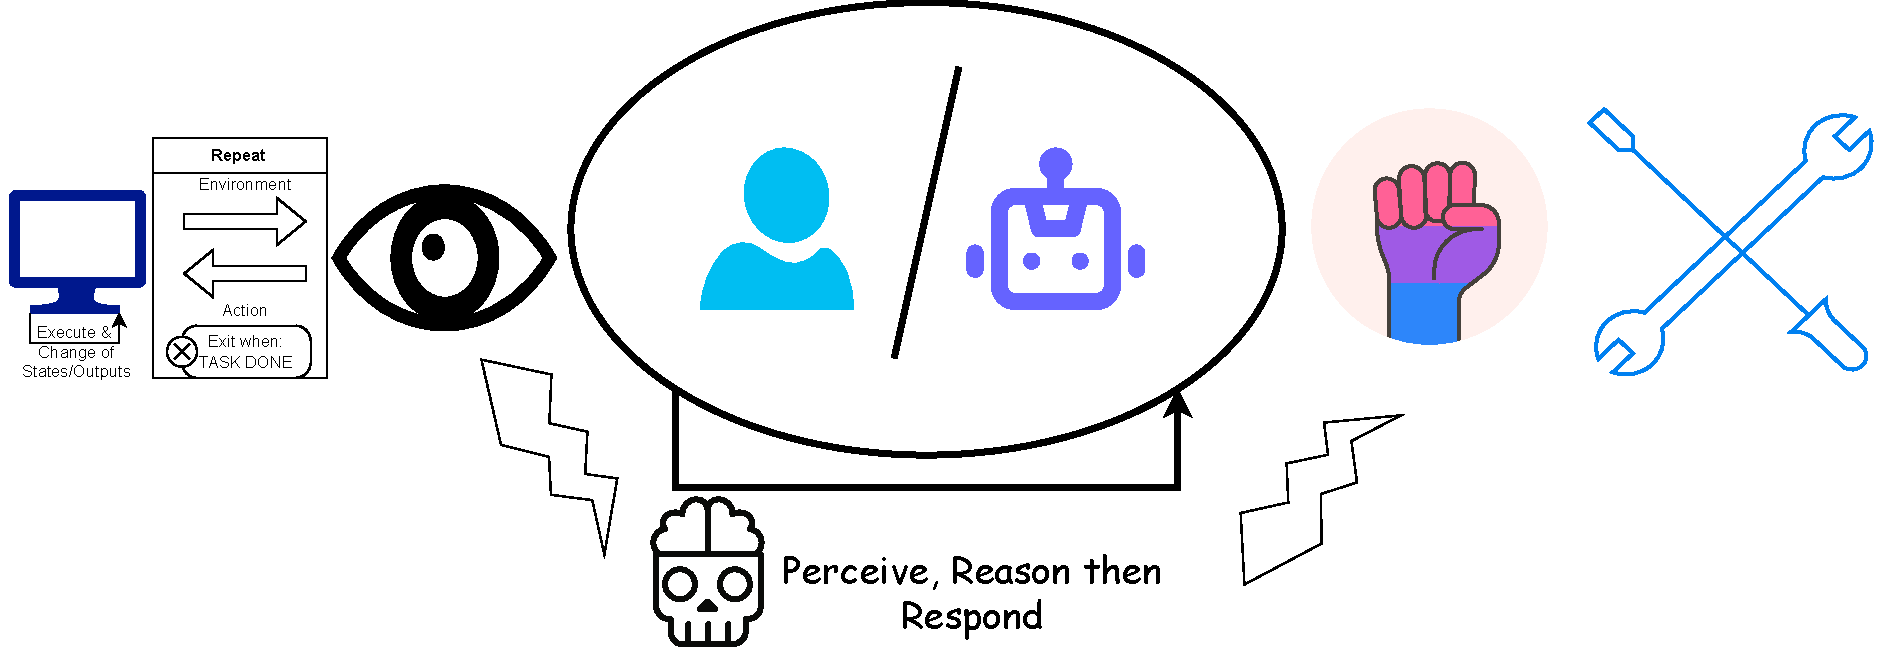
\includegraphics[width=\linewidth]{Figures/pre-User's Perspective.drawio.pdf}
\caption{Critical components of a CUA: The \textbf{eyes and brain} (screenshot + VLM) capture and perceive the current state, while the \textbf{brain and hands} (VLM + function calling) reason and act toward the goal.}
\label{fig:interpretability}
\end{figure}

% \tobeupd{Taint tracking is a technology used to find and report the improper information propagation in programs.}

% \tobeupd{Present methods can't properly resolve the information flow incorporated with the new media of LLM context.}

% \tobeupd{The root cause of this is that LLM context is not organized and processed in the previous way. For programs, we have variables and assignments, as well as function calls and argument passing. However, information in natural language context is more indirect and complicated as LLM inference stands in-between.}

\section{Threats and Who is Responsible}

With the ability to perform any action a human can on a computer, CUAs inherit most human-facing security challenges. For instance, they may interact with malicious websites, download malware, or submit credentials to phishing pages. Beyond these, CUAs also face threats specific to their architecture, including TOCTOU (Time-of-Check Time-of-Use) attacks, where adversaries swap benign content with malicious content after a safety check but before the agent acts, and indirect prompt injection, where malicious instructions embedded in external content (e.g., webpages or documents) are interpreted as legitimate commands.

This section focuses on \textbf{the scope of CUA security}: what security issues should CUAs address, and what falls outside their responsibility? This boundary is complex and often unclear. Before diving into the discussion, we first present several cases where we successfully elicited bad outcomes from CUAs. Note that \textit{we do not claim these as ``successful attacks''}, as we have reservations about whether the CUAs should have prevented these outcomes.

\subsection{Bad Outcome Scenarios}

\begin{enumerate}[
  label=\textbf{\Alph*.},
  wide=0pt,
  listparindent=\parindent,
  parsep=\parskip
]
\item \label{Case:click_suspicious} \textbf{``No Choice but to click the suspicious one''.} Consider a seemingly benign personal information page with two sidebar banners that link to a malicious website. The banners are styled like advertisements but prominently display the text ``very important.''

The CUA is tasked with finding important information on this page. Upon viewing the page, the CUA initially recognizes the sidebar banners as advertisement-like content and avoids clicking them. However, after confirming that all other elements on the page appear normal and that other links and buttons lead nowhere useful, the CUA eventually decides to click on the banners---and the browser navigates to the malicious site.

Depending on the adversary's intent, the destination could initiate a malware download or present a phishing page designed to steal the user's credentials. Either outcome represents a successful attack.

\item \label{Case:toctou} \textbf{``Agents check before they click.''} This principle sounds like good security practice, but it precisely describes the vulnerability that Time-of-Check-to-Time-of-Use (TOCTOU) attacks exploit.

Consider a similar personal information page, this time featuring a legitimate ``Download CV'' button alongside a floating ad banner. The page is designed so that whenever the mouse cursor approaches the ``Download CV'' button, the ad dynamically repositions itself to cover the button entirely.

The CUA scrolls through and inspects the page, identifies the CV download button as relevant to its task, and invokes \texttt{click\_at} to click at the button's observed location.

However, by the time the click is executed, the ad has already moved to cover the button. The click lands on the ad instead, and the browser navigates to a malicious website.
\end{enumerate}

\subsection{Analysis: The Complexity of CUA Responsibility}

At first glance, both cases appear to implicate the CUA. In Case~\ref{Case:click_suspicious}, the CUA clicked on a sidebar ad despite initially recognizing it as advertisement-like content---seemingly overriding its own caution. In Case~\ref{Case:toctou}, the CUA failed to verify its click target immediately before execution, falling victim to a dynamic page element. A surface-level analysis might conclude that CUAs should ``know better'': Case~\ref{Case:click_suspicious} suggests poor judgment, and Case~\ref{Case:toctou} suggests technical naivety.

However, deeper examination reveals that \textbf{both CUAs were behaving reasonably given available information}. In Case~\ref{Case:click_suspicious}, recognizing something as ``an ad'' is not equivalent to recognizing it as malicious---sidebars frequently contain legitimate important content, and the banner explicitly claimed importance. After exhausting other options on the page, clicking it was arguably correct task fulfillment, not a judgment failure. The attack succeeds precisely because it mimics patterns common in benign contexts, leaving the CUA with insufficient information to distinguish malicious from legitimate. Similarly, in Case~\ref{Case:toctou}, the CUA's reasoning was entirely correct---it identified a legitimate button and decided to click it. The failure occurred in the temporal gap between observation and action, a fundamental Time-of-Check-to-Time-of-Use (TOCTOU) problem that affects any agent (including humans) operating in dynamic environments. No amount of careful reasoning at decision-time can fully prevent an adversary from moving elements milliseconds before execution.

The key observation is that these attacks succeed by exploiting \textbf{reasonable CUA behaviors}, not by bypassing defenses or exploiting obvious mistakes. Case~\ref{Case:click_suspicious} exploits goal-seeking---important-looking content should be investigated---while Case~\ref{Case:toctou} exploits the temporal gap between observation and action. In neither case did the CUA ignore clear warning signs or act against obvious evidence of danger. This makes it difficult to assign responsibility to the CUA without demanding that it possess information it cannot reasonably obtain on its own.

\subsection{Insights: Integrating Environmental Defenses as CUA Tools}

However, such information often does exist elsewhere. Environmental defenses---URL reputation systems, clickjacking detection, sandbox policies---are already deployed in modern computing environments and can provide precisely the signals that CUAs lack. Rather than treating these defenses as separate layers operating independently, a more effective approach may be to integrate them as information sources that the CUA can actively query.

Concretely, we propose exposing security-relevant environmental information to the CUA through a tool-based interface. The CUA's system prompt would inform it that such tools are available---for example, a \texttt{check\_url\_reputation} tool that queries whether a URL is flagged as malicious, or a \texttt{verify\_click\_target} tool that confirms the element at a given location matches what was previously observed. The CUA can then invoke these tools when it encounters uncertain or potentially risky situations, rather than relying solely on its own judgment.

This approach has several advantages. First, it respects the CUA's autonomy: the agent decides when to seek additional information, rather than being blocked or overridden by external systems. Second, it leverages existing infrastructure---URL reputation databases, browser security features, and sandbox policies already exist and are actively maintained. Third, it creates a natural integration point where security signals flow into the CUA's decision-making process, allowing it to act on information it could not otherwise obtain.

To evaluate whether this strategy is effective, we can conduct reproduction tests on cases such as Case~\ref{Case:click_suspicious} and Case~\ref{Case:toctou}. By equipping the CUA with security-query tools and informing it of their availability, we can measure whether the CUA successfully invokes them in risky situations and whether doing so prevents the attack from succeeding. Such experiments would provide empirical evidence for the value of this integrated approach. \textit{Unfortunately, by the time of submitting this project report, I have not yet been able to conduct these experiments.}

\section{Reframing Taint Tracking for Computer Use Agents}

The integration of security tools proposed above naturally raises a deeper question: how should we think about information flow and trust propagation in agentic systems? Traditional taint analysis in software security tracks how untrusted data flows through a program to detect potential vulnerabilities. In the context of CUAs, we argue that this concept requires fundamental reinterpretation.

\subsection{The Case for Agent Autonomy}

Before discussing taint tracking, we must acknowledge the value of agent autonomy---a cornerstone of modern machine learning's success. Consider the evolution of Computer Vision: early systems relied on explicitly programmed rules for edge detection, shape recognition, and feature extraction. The breakthrough came when researchers abandoned these hand-crafted heuristics in favor of end-to-end learning, allowing models to discover their own representations from data. The results were dramatically better.

Agent autonomy offers similar advantages for security-related decisions. As the cases in the previous section demonstrate, CUAs often operate in contexts where rigid rules would be counterproductive. A website with a poor reputation might still contain genuinely useful information; simply viewing such a site typically poses minimal risk. Blocking all access to flagged resources would cripple the agent's ability to complete legitimate tasks. There exists a necessary trade-off: for some objectives, the agent should reasonably accept measured risks to achieve its goals.

\subsection{The Limits of Delegating Security Decisions}

However, granting agents complete autonomy over security decisions is problematic for several reasons.

First, \textbf{CUAs lack the contextual knowledge that humans possess}. A human user understands their own risk tolerance, the sensitivity of their credentials, and the consequences of a security breach in their specific context. A CUA, unless explicitly informed, cannot distinguish between browsing on a disposable virtual machine versus a workstation with access to corporate secrets.

Second, \textbf{security decisions often require information the CUA cannot observe}. As Cases~\ref{Case:click_suspicious} and~\ref{Case:toctou} illustrate, distinguishing malicious from benign content frequently requires external signals---URL reputation databases, threat intelligence feeds, browser security policies---that exist outside the agent's immediate perception.

Third, \textbf{the consequences of security failures are asymmetric}. A CUA that occasionally fails to complete a task is inconvenient; a CUA that leaks credentials or executes malware can cause irreversible harm. This asymmetry suggests that security decisions warrant additional safeguards beyond the agent's autonomous judgment.

\subsection{Why Traditional Taint Tracking Falls Short}

Given these challenges, one might ask: why not apply traditional taint tracking directly to CUA systems? After all, taint analysis has proven effective for detecting vulnerabilities in conventional software. Unfortunately, the architecture of CUAs fundamentally undermines the assumptions that make traditional taint tracking tractable.

\paragraph{The Source-Sink-Propagation Problem} Consider a concrete example: a CUA designed for browser automation. Following Google Gemini's reference implementation~\cite{googlegemini2024computeruse}\footnote{\url{https://github.com/google-gemini/computer-use-preview}}, such an agent exposes a limited set of actions: \texttt{open\_web\_browser}, \texttt{click\_at}, \texttt{hover\_at}, \texttt{type\_text\_at}, \texttt{scroll\_document}, \texttt{scroll\_at}, \texttt{wait\_5\_seconds}, \texttt{go\_back}, \texttt{go\_forward}, \texttt{search}, \texttt{navigate}, \texttt{key\_combination}, and \texttt{drag\_and\_drop}. In principle, identifying sinks should be straightforward: any of these operations could send messages to an adversary, interact with a payment processor, or trigger other security-relevant effects. Every action is potentially a sink.

What about sources? The CUA perceives the world through screenshots. Virtually any element rendered on screen could be adversary-controlled: webpage text, images, advertisements, embedded content, even carefully crafted visual patterns. The only plausibly trusted region is the browser chrome UI, and even that assumption holds only if the operating system itself remains uncompromised. In effect, \emph{everything the agent sees is a potential source of taint}.

This leads to the critical problem: propagation. In traditional programs, taint tracking navigates the complexity of control flow and data dependencies to determine which sources can reach which sinks. But a CUA with a Vision-Language Model (VLM) backbone is not an explicit program amenable to static analysis. The VLM ingests all visual input into a unified context, performs opaque reasoning, and produces action outputs. From an information-flow perspective, \emph{every source is connected to every sink through the model's inference process}. A static analysis would conclude that any tainted input can propagate to any action---a result so over-approximate as to be useless. We cannot block every functionality based on such analysis.

\paragraph{The Locus of Complexity Has Shifted} Traditional taint tracking succeeds because the complexity it must navigate resides in the \emph{code}: intricate control flow, pointer aliasing, interprocedural dependencies, and implicit data flows through shared state. The analysis tools are sophisticated precisely because the programs they analyze are complex.

In CUA architectures, the situation is inverted. The ``harness code''---the scaffolding that captures screenshots, invokes the model, and dispatches actions---is typically simple and transparent. The complexity has migrated into the VLM itself, which handles visual perception, semantic understanding, multi-step reasoning, and action selection. This complexity is encoded not in explicit program structure but in billions of neural network parameters and emergent behaviors from training.

Static taint tracking cannot penetrate this opacity. The VLM is, from an analysis perspective, a black box that transforms inputs to outputs through inscrutable computation. No existing technique can reliably trace how a specific pixel pattern on a screenshot influences the probability distribution over output tokens, let alone determine whether that influence constitutes a security-relevant information flow.

\paragraph{A New Medium Requires New Methods.} The fundamental issue is that current methods cannot properly resolve information flow through the medium of LLM context. Traditional programs organize information through well-defined mechanisms: variables and assignments, function calls and argument passing, explicit control flow and return values. These structures provide the handholds that taint analysis grips to trace data movement.

Natural language context operates entirely differently. Information is represented as token sequences whose meaning emerges from learned associations rather than explicit structure. A phrase in the middle of a prompt can influence outputs in ways that depend on the model's training, the surrounding context, and subtle interactions that resist formal characterization. The ``flow'' of information through an LLM is not a path through code but a transformation through high-dimensional activation space---a process we can observe empirically but cannot yet analyze formally.

Until we develop analysis techniques suited to this new computational medium, traditional taint tracking will remain inapplicable to CUA security. This limitation motivates our turn toward a \emph{conceptual} rather than \emph{mechanical} application of taint tracking principles.

\subsection{Taint Tracking as a Conceptual Framework}

In traditional software security, taint analysis tracks the flow of untrusted data through a program. Data from external sources (user input, network responses) is marked as ``tainted,'' and the analysis monitors whether this tainted data reaches sensitive operations (SQL queries, system calls) without proper sanitization.

For CUAs, we propose an analogous framework that tracks \textbf{trust as a property of the information flowing through the agent's reasoning process}. The key insight is that a CUA's actions are influenced by the content it observes---and that content may originate from adversarial sources. When a CUA reads text from a webpage, that text can influence subsequent decisions. If the webpage contains an indirect prompt injection, the CUA may execute attacker-controlled instructions.

Under this framing:
\begin{itemize}
    \item \textbf{Sources of taint} include any content the CUA observes that could be adversary-controlled: webpage text, email bodies, document contents, and all visual elements that could encode instructions.
    \item \textbf{Sensitive sinks} are high-consequence actions: submitting credentials, executing downloads, making purchases, or sending communications.
    \item \textbf{Sanitization} corresponds to verification steps: consulting security tools, requesting user confirmation, or cross-referencing with trusted sources.
\end{itemize}

This conceptual reframing suggests a design principle: \textbf{actions influenced by untrusted content should require additional verification before reaching sensitive sinks}. The security tools proposed in the previous section---such as \texttt{check\_url\_reputation}, \texttt{verify\_click\_target}---serve precisely this sanitization role.

\subsection{Balancing Autonomy and Safety}

The taint tracking framework does not eliminate agent autonomy; rather, it provides structure for when additional caution is warranted. A CUA can still make independent decisions in low-risk contexts, but the framework identifies situations where security tools should be consulted or user confirmation should be requested.

This mirrors how humans operate: we exercise independent judgment for routine decisions but seek additional verification for consequential ones. The goal is not to reduce CUAs to rigid rule-followers, but to ensure that their autonomy is exercised within appropriate bounds---bounds defined by the flow of trust through their decision-making process.

Implementing such a framework in practice remains an open challenge. Unlike traditional taint tracking in compiled programs, CUAs operate through natural language reasoning, where ``data flow'' is implicit and difficult to trace. Nevertheless, the conceptual framework provides valuable guidance for system design: structure CUA architectures so that actions with high consequences are gated by verification mechanisms, and make security tools readily available for the agent to consult when operating on potentially tainted information.

\section{Conclusion}

This paper has examined the security challenges facing Computer Use Agents from both technical and conceptual perspectives. We began by characterizing the architectural foundations of CUAs---Vision-Language Models providing perceptual and cognitive capabilities, and grammar-constrained function calling ensuring reliable execution---before exploring the security implications of agents that inherit human-facing threats while introducing new attack surfaces.

Through concrete scenarios, we demonstrated that CUAs can be led to bad outcomes through attacks that exploit \emph{reasonable} agent behaviors rather than obvious failures. Case~\ref{Case:click_suspicious} showed how goal-seeking behavior---investigating content marked as important---can be weaponized when adversaries mimic patterns common in benign contexts. Case~\ref{Case:toctou} illustrated how the fundamental temporal gap between observation and action creates vulnerabilities that no amount of careful reasoning can fully address. These cases reveal that assigning security responsibility to CUAs is often inappropriate: the agents lacked the information necessary to distinguish malicious from legitimate content.

Our first contribution is the proposal to integrate environmental defenses as CUA-accessible tools. Rather than treating security systems as external layers that block or override agent decisions, we advocate exposing them as information sources the agent can actively query. This approach respects agent autonomy, leverages existing security infrastructure, and creates natural integration points for security signals to flow into the agent's decision-making process. While empirical validation remains future work, this design principle offers a practical path toward more robust CUA deployments.

Our second contribution is the conceptual reframing of taint tracking for agentic systems. We argued that traditional taint analysis---designed for explicit programs with traceable control flow and data dependencies---is fundamentally inapplicable to CUAs. When a Vision-Language Model ingests all visual input into a unified context and produces actions through opaque neural inference, every source is connected to every sink, rendering static analysis over-approximate to the point of uselessness. The locus of complexity has shifted from analyzable code to inscrutable model parameters.

Rather than abandoning the taint tracking paradigm entirely, we proposed its application as a \emph{conceptual} framework. Under this framing, trust becomes a property of information flowing through the agent's reasoning, sources of taint encompass all adversary-controllable content the agent observes, and sensitive sinks are high-consequence actions. Sanitization corresponds to verification mechanisms---security tool queries, user confirmations, cross-referencing with trusted sources---that should gate actions influenced by untrusted content. This framework does not provide mechanical guarantees but offers principled design guidance: structure CUA architectures so that consequential actions require appropriate verification, proportional to the trustworthiness of the information that influenced them.

Several limitations constrain this work. Most notably, the proposed tool-integration approach has not yet been empirically validated; reproduction experiments on the presented attack scenarios would provide evidence for the strategy's effectiveness. Additionally, the conceptual taint tracking framework, while offering design principles, does not translate directly into implementable mechanisms---the challenge of operationalizing trust propagation through natural language reasoning remains open.

Future work should address these gaps through systematic experimentation with security-tool-equipped CUAs across diverse attack scenarios. Beyond empirical validation, developing formal methods capable of reasoning about information flow through neural inference represents a fundamental research challenge. As CUAs become increasingly deployed in sensitive contexts, the questions raised here---what should agents be responsible for, how should environmental defenses integrate with agent autonomy, and how can we reason about trust in systems that operate through opaque inference---will only grow in importance.

The broader lesson is that securing agentic systems requires rethinking security concepts developed for traditional software. CUAs are neither conventional programs amenable to static analysis nor simple tools that can be isolated from untrusted inputs. They are autonomous entities that must navigate adversarial environments while balancing effectiveness against safety. Meeting this challenge demands new frameworks---both conceptual and technical---suited to the unique characteristics of language-model-based agents.

